\chapter{Introduction}

\section{Context and Motivation}
\paragraph{}
% fingerprint
A traditional door lock with a key or a door lock with fingerprint integrated is a standard security solution. It is still the most reliable and fast solution since the early days. Because each lock key has different spring-loaded pins in the cylinder, it requires a specific key to push the pins inside the lock body. We all have to touch fingers to that surface as a traditional door lock or a newer lock with a numeric pad or fingerprint, and this will make it like a mediate surface for the virus to stay.

\begin{figure}[H]
    \centering
    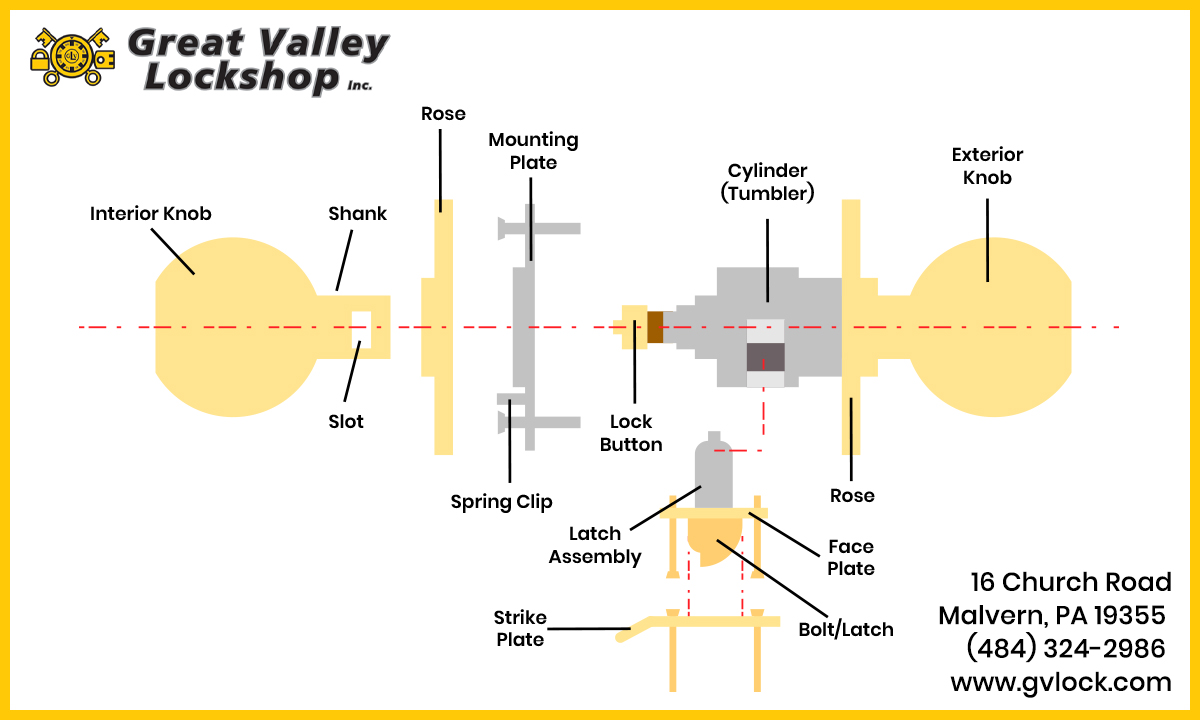
\includegraphics[scale=1.2]{Cylinder-Lock-Diagram.jpeg}
    \caption{Diagram showing the inside of a door lock}
    \caption*{\textit{source: gvlock.com}}
    \label{fig:doorLock}
\end{figure}

\acrlong{covid-19} is the most dangerous infectious disease in the last three years. From the first case in Wuhan City, China, it is a severe pandemic throughout the world. Max Roser, Hannah Ritchie, Esteban Ortiz-Ospina, and Joe Hasell\cite{owidcoronavirus} indicate that from late 2019, there are 176 million confirmed cases, with 3.81 million deaths. In Vietnam, as we experienced in the \acrshort{sars} epidemic in 2003, the situation here is in control now. However, since the pandemic is still a big problem outside Vietnam, according to Havard Health Publishing\cite{harvard_health_publishing_2021}, we should clean frequently touched objects and surfaces regularly and wash our hands often with soap and water. An early stage of prevention is essential in order not to have another outbreak here.

% face recognition
On the other hand, face recognition will solve the problem. As we do not have to touch any surface to verify that we are granted to open the lock, just a simple step is to look at the camera. The hard part is for the local server with a deep learning model to compare the face with a local database.

\begin{figure}[H]
    \centering
    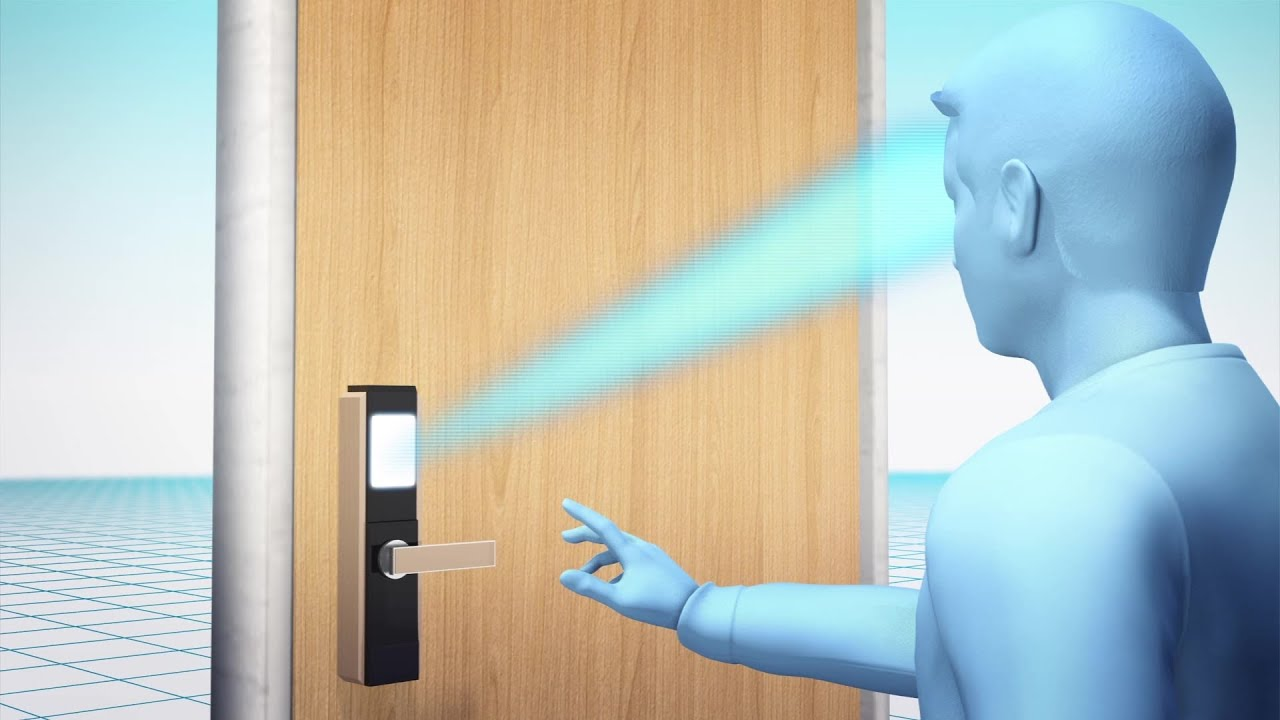
\includegraphics[scale=0.29]{faceRecognitionDemo.png}
    \caption{Door lock integrated with face recognition}
    \label{fig:faceregDoorLock}
\end{figure}

As usual, many researchers in face recognition objects choose to train a model with a large of images for each class. This consumes much time, power to train, and we must re-train the model from scratch if a new person comes. Meanwhile, following to Florian Schroff et al.\cite{DBLP:journals/corr/SchroffKP15} choosing to follow the one-shot learning method can decrease the training model time, which benefits a scale-up in the future. 
\clearpage
\section{Objectives}
\paragraph{}
The main topic of this internship is to improve the accuracy of the deep learning model to classify Asian faces better based on the pre-trained weights on the LFW dataset. It also applies IoT devices for hand-less control for domestic usage and integrates with attendance checks for household and industrial usage. Our goal after the internship is to study and use \acrshort{iot} connectivity, combined with a deep learning model to create a product that uses face recognition to validate if the person is granted to open the door and control smart home devices so that they can do it without hand touch.

The main objectives of this internship include:

\begin{itemize}
    \item Study knowledge of \acrlong{cnn} and implement it on a pre-trained FaceNet\cite{DBLP:journals/corr/SchroffKP15} model.
    \item Propose to apply the Asian dataset to the face recognition model for better performance on recognizing Vietnamese.
    \item Study knowledge of IoT connectivity
\end{itemize}

\section{Thesis Organization}
This report is organized as follows:
\begin{enumerate}
	\item Materials and Methods: presents our dataset, proposed methodology, and the evaluation scenario.
	\item Result and Discussion: presents the evaluation results and discusses our results.
	\item Conclusion and Future-work: conclude the work and presents future research directions.
\end{enumerate}